% Options for packages loaded elsewhere
\PassOptionsToPackage{unicode}{hyperref}
\PassOptionsToPackage{hyphens}{url}
%
\documentclass[
]{article}
\usepackage{lmodern}
\usepackage{amsmath}
\usepackage{ifxetex,ifluatex}
\ifnum 0\ifxetex 1\fi\ifluatex 1\fi=0 % if pdftex
  \usepackage[T1]{fontenc}
  \usepackage[utf8]{inputenc}
  \usepackage{textcomp} % provide euro and other symbols
  \usepackage{amssymb}
\else % if luatex or xetex
  \usepackage{unicode-math}
  \defaultfontfeatures{Scale=MatchLowercase}
  \defaultfontfeatures[\rmfamily]{Ligatures=TeX,Scale=1}
\fi
% Use upquote if available, for straight quotes in verbatim environments
\IfFileExists{upquote.sty}{\usepackage{upquote}}{}
\IfFileExists{microtype.sty}{% use microtype if available
  \usepackage[]{microtype}
  \UseMicrotypeSet[protrusion]{basicmath} % disable protrusion for tt fonts
}{}
\makeatletter
\@ifundefined{KOMAClassName}{% if non-KOMA class
  \IfFileExists{parskip.sty}{%
    \usepackage{parskip}
  }{% else
    \setlength{\parindent}{0pt}
    \setlength{\parskip}{6pt plus 2pt minus 1pt}}
}{% if KOMA class
  \KOMAoptions{parskip=half}}
\makeatother
\usepackage{xcolor}
\IfFileExists{xurl.sty}{\usepackage{xurl}}{} % add URL line breaks if available
\IfFileExists{bookmark.sty}{\usepackage{bookmark}}{\usepackage{hyperref}}
\hypersetup{
  pdftitle={Local Climate Zone classification in mega urban areas using Landsat images and random forests: A case study of Hong Kong},
  pdfauthor={Ericka B. Smith},
  hidelinks,
  pdfcreator={LaTeX via pandoc}}
\urlstyle{same} % disable monospaced font for URLs
\usepackage[margin=1in]{geometry}
\usepackage{graphicx}
\makeatletter
\def\maxwidth{\ifdim\Gin@nat@width>\linewidth\linewidth\else\Gin@nat@width\fi}
\def\maxheight{\ifdim\Gin@nat@height>\textheight\textheight\else\Gin@nat@height\fi}
\makeatother
% Scale images if necessary, so that they will not overflow the page
% margins by default, and it is still possible to overwrite the defaults
% using explicit options in \includegraphics[width, height, ...]{}
\setkeys{Gin}{width=\maxwidth,height=\maxheight,keepaspectratio}
% Set default figure placement to htbp
\makeatletter
\def\fps@figure{htbp}
\makeatother
\setlength{\emergencystretch}{3em} % prevent overfull lines
\providecommand{\tightlist}{%
  \setlength{\itemsep}{0pt}\setlength{\parskip}{0pt}}
\setcounter{secnumdepth}{5}
\usepackage{setspace}\linespread{1.5}
\usepackage{booktabs}
\usepackage{longtable}
\usepackage{array}
\usepackage{multirow}
\usepackage{wrapfig}
\usepackage{float}
\usepackage{colortbl}
\usepackage{pdflscape}
\usepackage{tabu}
\usepackage{threeparttable}
\usepackage{threeparttablex}
\usepackage[normalem]{ulem}
\usepackage{makecell}
\usepackage{xcolor}
\ifluatex
  \usepackage{selnolig}  % disable illegal ligatures
\fi

\title{Local Climate Zone classification in mega urban areas using
Landsat images and random forests: A case study of Hong Kong}
\author{Ericka B. Smith}
\date{Winter 2021}

\begin{document}
\maketitle

\hypertarget{introduction}{%
\section{Introduction}\label{introduction}}

\hypertarget{background}{%
\subsection{Background}\label{background}}

The population worldwide is increasing and urbanizing (United Nations et
al., 2019). In addition, issues surrounding environmental change and
pollution are exacerbated in cities (Bechtel et al., 2015) (Santamouris,
2020). These changes compound the effects of each other and, as a
result, a greater understanding of these processes is more important now
than ever before (Bechtel et al., 2015).

Urban Heat Islands, where urban areas are warmer than the neighboring
rural areas, are of particular concern. This is for four primary
reasons: increased energy consumption, elevated emissions of air
pollutants and greenhouse gasses, compromised human health and comfort,
and impaired water quality (US EPA, 2014). A multitude of processes
combine to cause Urban Heat Islands. Broadly speaking, urban built
structures hold more heat than the structures and vegetation in
surrounding areas (Hibbard et al., 2017). In particular, cities have an
overabundance of impervious surfaces, along with a lack of vegetation
(Hibbard et al., 2017). Knowledge about microclimates within cities,
especially in the context of prospective sites for climate risk
adaptation efforts, has the potential to ease some of these disturbances
(Lempert et al., 2018) .

Unfortunately, information on these sites can be difficult to obtain.
Though there is a plethora of satellite imagery, the current methods to
classify this imagery are not always accurate. (Yokoya et al., 2018).
Historically the focus was on the broad categories of urban vs.~rural,
which does not give enough information about the nuanced climate within
a large urban area (Stewart \& Oke, 2012). Local Climate Zone (LCZ)
classification was created by Stewart and Oke (2012) (Figure 1) to
alleviate this problem, but it often requires a significant investment
from individuals with specialist knowledge to successfully classify a
city (Bechtel et al., 2015). Even the best models have low accuracy
outside of their training city (Verdonck et al., 2017) (Yokoya et al.,
2018). Therefore, this issue with generalizing a model to other cities,
transferability, is a topic of great interest in current Urban Heat
Island research (Tuia et al., 2017) (Yokoya et al., 2018).

\begin{figure}[H]

{\centering 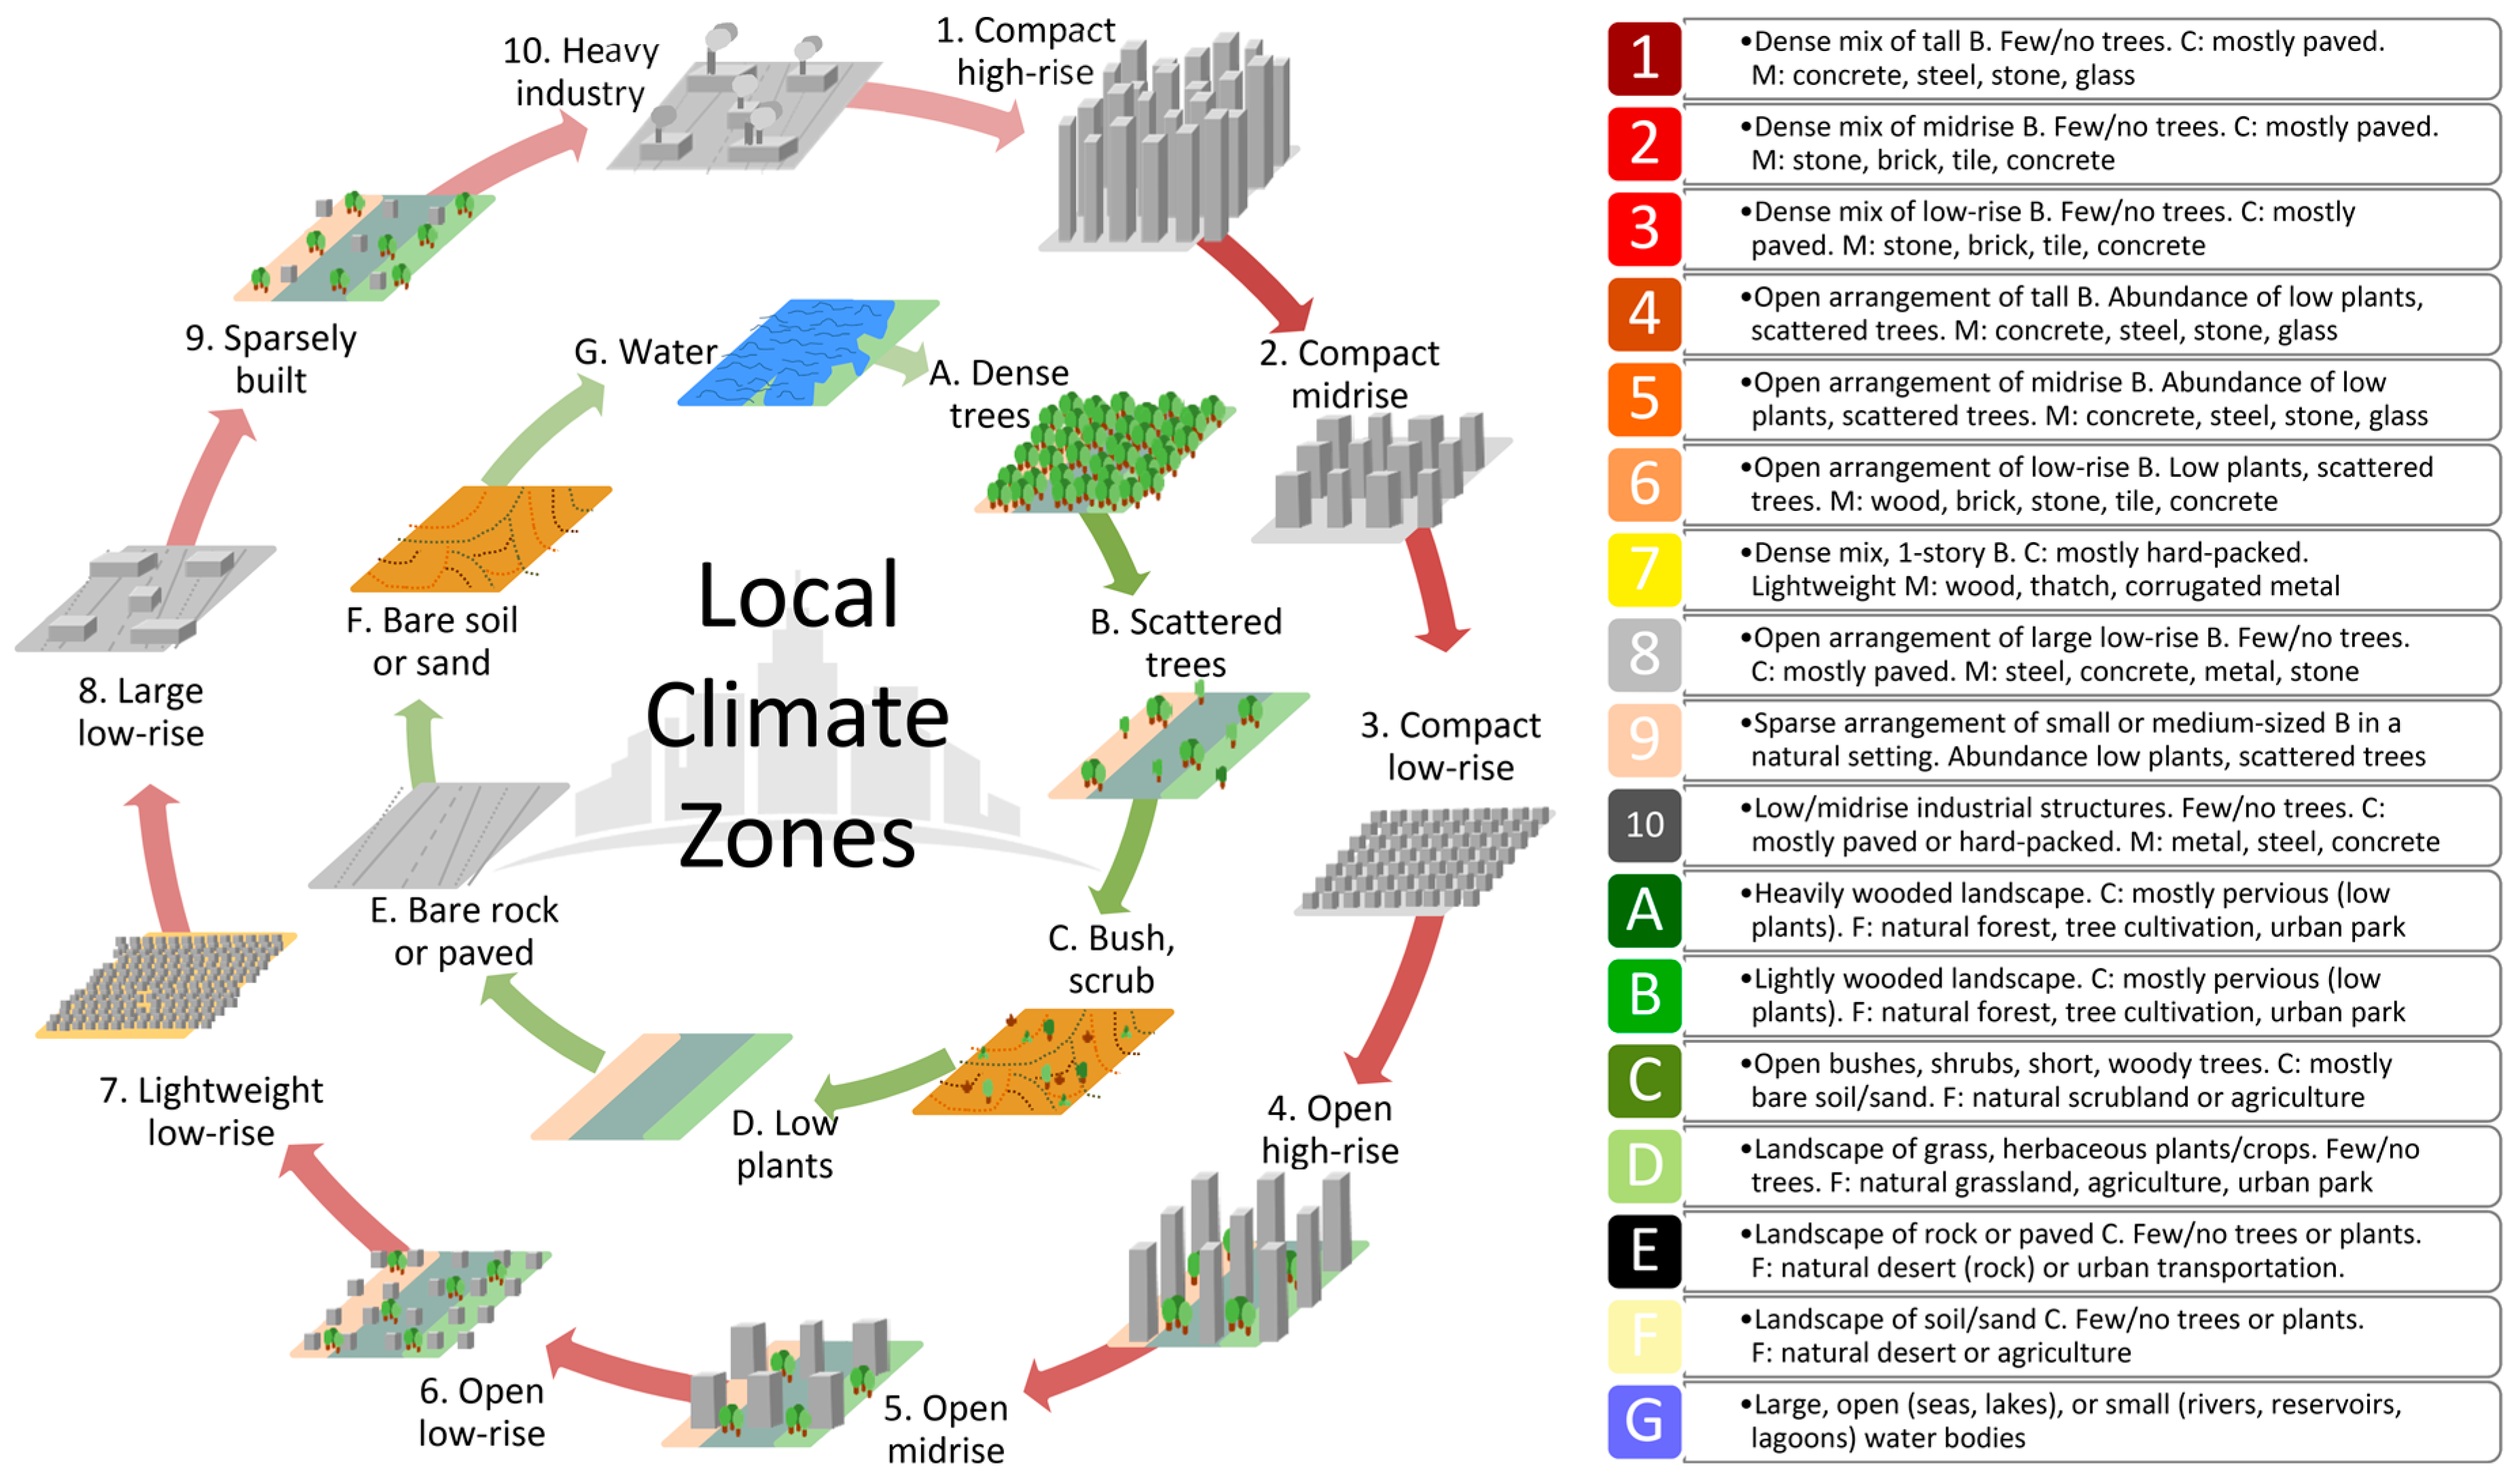
\includegraphics[width=1\linewidth]{figure_from_Bechtel_et_al_Stewart_Oke_cc-by4} 

}

\caption{Local Climate Zone classes. Originally from Stewart and Oke (2012) and remade by Bechtel et al. (2017). Copyright CC-BY 4.0}\label{fig:image-ref-for-in-text0}
\end{figure}

\hypertarget{objective}{%
\subsection{Objective}\label{objective}}

The goal of this project is to recreate aspects of the article
Comparison between convolutional neural networks and random forest for
local climate zone classification in mega urban areas using Landsat
images (Yoo et al., 2019), where methods for predicting LCZ classes for
four large cities throughout the world were compared. To do so, a small
training dataset from the 2017 Institute of Electrical and Electronics
Engineers (IEEE) Geoscience and Remote Sensing Society (GRSS) Data
Fusion Contest (Tuia et al., 2017) was used as ground truth for LCZ
classes. This was combined with satellite input data to create a series
of models, which were then compared to a larger, full LCZ layer for each
city and assessed for accuracy. The primary types of models considered
in the Yoo et al.~(2019) work were random forests and convolutional
neural networks. However, for this project the focus will be only on
random forests. In addition, rather than four cities, this investigation
will focus on just Hong Kong. This city was chosen due to its lack of
``red-star classes'' (LCZ classes with 3 or fewer polygons) in the study
area. The red-star classes add complexity to the splitting up of the
data into training and test sets. Since they by nature address only rare
classes, this complexity was deemed unnecessary for this project.
Finally, here;, a classification scheme like the one used by the World
Urban Database and Access Portal Tools (WUDAPT) project, denoted as
Scheme 1 (S1) in Yoo et al.~(2019) will be the focus, with comparisons
between accuracy using a variety of tuning parameters.

\hypertarget{methods}{%
\section{Methods}\label{methods}}

\hypertarget{data}{%
\subsection{Data}\label{data}}

Data for this analysis was accessed from the 2017 IEEE GRSS Data Fusion
Contest. Only the Hong Kong LCZ reference and Landsat 8 datasets were
used.

The LCZ reference data from the contest set was taken from the WUDAPT
database, checked for correctness, and then provided as a 100m
resolution raster layer. In this provided layer the LCZ classes are
numbered 1-17, rather than 1-10 and A-G, and initial inspection of the
data verified that numbers 11-17 directly match classes A-G. In Yoo et
al.~(2019) the first step they took with the reference data was randomly
dividing the polygons of each class into training and testing groups.
This required some preprocessing since I only had access to the data in
raster form and without any sort of polygon identification. Pixels
within the same polygon cannot be put into both training and validation
groups because it will artificially increase accuracy metrics (Zhen et
al., 2013).

In Yoo et al.~(2019) they downloaded and preprocessed their own Landsat
8 data to facilitate some of their classification schemes, but the
contest data was sufficient for the narrower scope of this project. The
Landsat 8 data provided by the contest includes four different dates, or
``scenes,'' each of which were downloaded from the USGS EarthExplorer
portal. Then the atmospheric band (band 9) and the panchromatic band
(band 8) were left out, and the data were resampled using the area
weighted average to 100 m x 100 m grids (Yokoya et al., 2018). To get
these data into a usable format they were loaded into R by band (each
band is a separate raster layer) and stacked by scene. All the scenes
were then stacked with the LCZ reference data and converted to a
dataframe, ready to be used as input data.

All 9 available bands of all 4 Landsat scenes amounted to 36 input
variables. Each pixel is an observation, with 279,312 pixels total over
the almost 2,800 square kilometers that are contained within the area of
interest. The LCZ reference data has 179 polygons, which cover 8,846
pixels. This is approximately 88.5 square kilometers and 3\% of the
total area of interest. The LCZ reference data was randomly split into
training and test sets by LCZ class and polygon. The resulting groups
are not exactly equal in pixel numbers, but I determined that
randomization of polygons takes precedence over equality in pixels due
to the potential for artificially high accuracy values, as mentioned
before. In order to get as close as possible a barplot was made showing
the number of pixels in training and test, by class, so that equality in
pixel number could be explored without having knowledge of polygon
groupings. Sampling was repeated until these bars looked marginally
even. (Table 1).

\begin{table}[H]

\caption{\label{tab:unnamed-chunk-1}Delineation of training and test data by polygon and pixel.}
\centering
\fontsize{8}{10}\selectfont
\begin{tabular}[t]{lll}
\toprule
Local Climate Zone & Train & Test\\
\midrule
\cellcolor{gray!6}{Class 1: Compact high-rise} & \cellcolor{gray!6}{13        (295)} & \cellcolor{gray!6}{13 (336)}\\
Class 2: Compact mid-rise & 6        (117) & 5 (62)\\
\cellcolor{gray!6}{Class 3: Compact low-rise} & \cellcolor{gray!6}{7        (185)} & \cellcolor{gray!6}{7 (141)}\\
Class 4: Open high-rise & 10        (275) & 9 (398)\\
\cellcolor{gray!6}{Class 5: Open mid-rise} & \cellcolor{gray!6}{4        (79)} & \cellcolor{gray!6}{4 (47)}\\
Class 6: Open low-rise & 6        (60) & 7 (60)\\
\cellcolor{gray!6}{Class 7: Lightweight low-rise} & \cellcolor{gray!6}{0        (0)} & \cellcolor{gray!6}{0 (0)}\\
Class 8: Large low-rise & 4        (90) & 5 (47)\\
\cellcolor{gray!6}{Class 9: Sparsely built} & \cellcolor{gray!6}{0        (0)} & \cellcolor{gray!6}{0 (0)}\\
Class 10: Heavy Industry & 4        (107) & 5 (112)\\
\cellcolor{gray!6}{Class 11: Dense trees} & \cellcolor{gray!6}{7        (762)} & \cellcolor{gray!6}{7 (854)}\\
Class 12: Scattered trees & 6        (194) & 7 (213)\\
\cellcolor{gray!6}{Class 13: Bush, scrub} & \cellcolor{gray!6}{4        (459)} & \cellcolor{gray!6}{5 (232)}\\
Class 14: Low plants & 6        (346) & 6 (222)\\
\cellcolor{gray!6}{Class 15: Bare rock or paved} & \cellcolor{gray!6}{0        (0)} & \cellcolor{gray!6}{0 (0)}\\
Class 16: Bare soil or sand & 0        (0) & 0 (0)\\
\cellcolor{gray!6}{Class 17: Water} & \cellcolor{gray!6}{5        (1266)} & \cellcolor{gray!6}{5 (1113)}\\
\bottomrule
\multicolumn{3}{l}{\textsuperscript{a} Number of polygons is listed first, with number of pixels in parentheses.}\\
\end{tabular}
\end{table}

\hypertarget{random-forests}{%
\subsection{Random Forests}\label{random-forests}}

Random forests consist of many decision trees. A decision tree can be
used for classification or regression. Here I will focus on
classification since my goal is to predict LCZ class, which is a
categorical variable. Decision trees put each observation through a
series of conditional statements, or splits, in order to group it with
other observations that are similar. These similar groups are expected
to have similar values for the predictor variable. Since the true value
of the predictor variable is known for the observations in the training
dataset, it is possible to measure the accuracy of each prospective
split, and therefore to build an optimal tree.

Each point in which the data could potentially be split into two groups
is called a node. The first split is called the root node. Nodes are
selected such that each one uses the conditional statement which subsets
the data into the best possible split. When any more subsetting does not
increase accuracy, the path ends, and this is called a leaf node. Any
nodes between the root node and leaf nodes are called internal nodes.

Splits are typically evaluated by Gini impurity or entropy. \[
\text{Gini Impurity} =\ I_G(t)\  = 1 - \sum_{i=1}^{C}p(i|t)^2
\] \[
\text{Entropy} =\ I_H(t)\ = -\sum_{i=1}^{C}p(i|t)\log_2p(i|t)
\] Where \(i\) is a class in the predictor variable, ranging from 1 to
\(C\). \(C\) is the total number of classes represented for a particular
node, \(t\). \(p(i|t)\) is the proportion of samples that belong to each
\(i\), for a particular node \(t\).

A Gini Impurity, or entropy, of 0 indicates a completely homogeneous
group, which cannot be improved upon. These metrics are used for
comparison: all possible variables and thresholds within those variables
are tried and their Gini impurity or entropy calculated, the variable
and threshold with the best (lowest) value selected for the node. This
is done recursively at each node until no split offers a decrease in the
metric of choice. The resulting collection of nodes is a decision tree.

Decision trees perform quite poorly with new samples. Including a
threshold value for the accuracy metric can help, as it keeps trees more
simple, but they are still prone to overfitting. Collecting them into a
random forest addresses this issue. True to its name, a random forest is
a collection of decision trees that have a component of randomness. The
predictive aspect of a random forest does not only rely on one tree, it
is determined by totaling up the decisions, or ``votes,'' that all of
the trees make.

Each tree is created individually and starts with bootstrapping the
training dataset. Then the process is similar to the one described above
for decision trees. However, for each node only a subset of the
variables are randomly selected and used as candidates to split up the
bootstrapped data. Not all the variables are used at each node because
doing so reduces correlation and introduces randomness into the model.
Whichever variable best splits the data will be the variable that is
kept at that node in that specific tree. This is either done recursively
until no more splits are beneficial (just as in a regular decision
tree), or until minimum size of the node is reached. To create the next
tree the process is the same, but starts completely over with a new
bootstrap sample of the training data. This is repeated for a chosen
number of trees.

This choice of the number of trees to create is a tuning parameter. Too
many trees can be computationally expensive, but too few can create a
model that is poor at prediction. Another important tuning parameter is
the choice of how many variables to randomly select at each node. The
default value for classification is typically the square root of the
number of variables, and for regression it is the number of variables
divided by three. Values for the minimum size of terminal nodes, which
is the minimum number of observations required to make a leaf node, can
also be varied. A large minimum size means smaller trees and faster
completion of the random forest. This is an alternate strategy for
controlling depth, which, in the randomForest package in R, cannot be
directly controlled. Depth indicates the number of splits a tree has.
Greater depth gives more information about the data. Another tuning
parameter with a similar approach is the maximum number of terminal
nodes a tree can have. Without setting this parameter, trees are grown
as large as possible.

To use a random forest to make predictions for a new set of input
values, the values are fed into each decision tree individually. The
predictions from each tree are combined either by direct vote (for
categorical variables) or an average (for quantitative variables) and
this becomes the final predicted result. This process is called bagging,
because it is the action of bootstrapping the data to create each tree
and using the aggregate to make a decision. Bagging is useful because it
reduces variance without introducing bias.

For this analysis, parameters were varied individually. This is limited
in that it does not explore any potential interactions, but beneficial
in that it is more clear the individual contribution of a parameter. The
number of trees is the primary parameter of interest, since reducing it
as much as possible can have a large impact on time and computational
resources required.

\hypertarget{accuracy-assessment}{%
\subsection{Accuracy Assessment}\label{accuracy-assessment}}

In line with the methods used in our reference paper and the remote
sensing field, accuracy metrics will be based on predictions for the
test dataset and will include the following: \[
\text{Overall Accuracy}= OA= \frac{\text{number of correctly classified reference sites}}{\text{total number of reference sites}}
\] \[
\text{Overall Accuracy in Urban Areas} = OA_{urb}\ = \frac{\text{number of correctly classified urban reference sites}}{\text{total number of urban reference sites}}
\] \[
\text{Overall Accuracy in Natural Areas}=OA_{nat}\ = \frac{\text{number of correctly classified natural reference sites}}{\text{total number of natural reference sites}}
\] \[
UA(z)\ = \frac{\text{number of correctly identified pixels in class z}}{\text{total number of pixels identified as class z}}
\] \[
PA(z) = \frac{\text{number of correctly identified pixels in class z}}{\text{number of pixels truly in class z}}
\] \[
F_1\text{ Score} = 2*\frac{UA*PA}{UA+PA}
\]

\hypertarget{results}{%
\section{Results}\label{results}}

\hypertarget{varying-the-parameter-for-number-of-trees}{%
\subsection{Varying the Parameter for Number of
Trees}\label{varying-the-parameter-for-number-of-trees}}

The parameter for the number of trees was initially varied between 5 and
500 at intervals of 5. The resulting overall accuracy metrics indicate a
leveling off around 125 trees (Figure 2). There's also a clear
distinction between accuracy in urban vs.~natural classes, with natural
classes having a much higher overall accuracy.

\begin{figure}[H]

{\centering 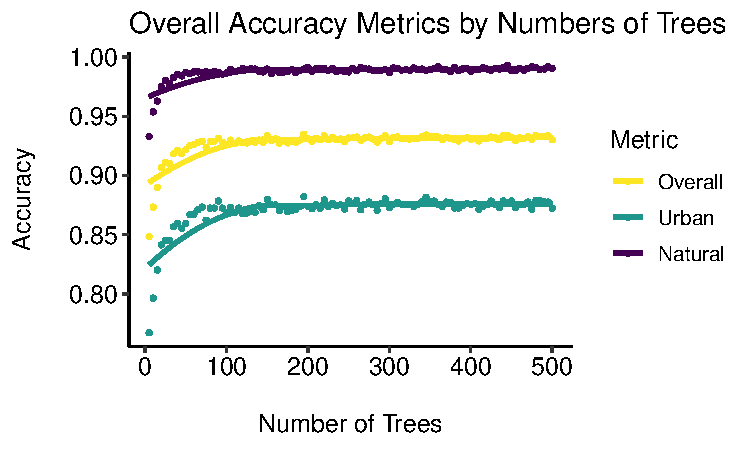
\includegraphics[width=0.75\linewidth]{../results/plots/ntree_5_to_500_line_plot} 

}

\caption{The increase in OA metrics levels off around 125 trees. Urban classes (1-10) have much lower accuracy than natural classes (11-17). These metrics were calculated based on the out-of-bag dataset.}\label{fig:image-ref-for-in-text1}
\end{figure}

The plot of F-1 scores (Figure 3) explores each class individually. It's
clear that there are three approximate groupings. The dense trees;
scattered trees; bush, scrub; low plants; and water classes (11, 12, 13,
14, and 17, respectively) have the highest F-1 scores throughout,
staying in the high 0.9 range almost irrespective of number of random
forest trees, though scattered trees (12) stands out as a little lower
than the others. The open low-rise, large low-rise, and heavy industry
classes (6, 8, and 10, respectively) have much lower F-1 scores which
are around 0.5 to 0.7. Finally, in the middle are the compact high-rise,
compact mid-rise, compact low-rise, open high-rise, and open mid-rise
classes (1-5, respectively), with F-1 scores hovering around 0.7 to 0.9.

\begin{figure}[H]

{\centering 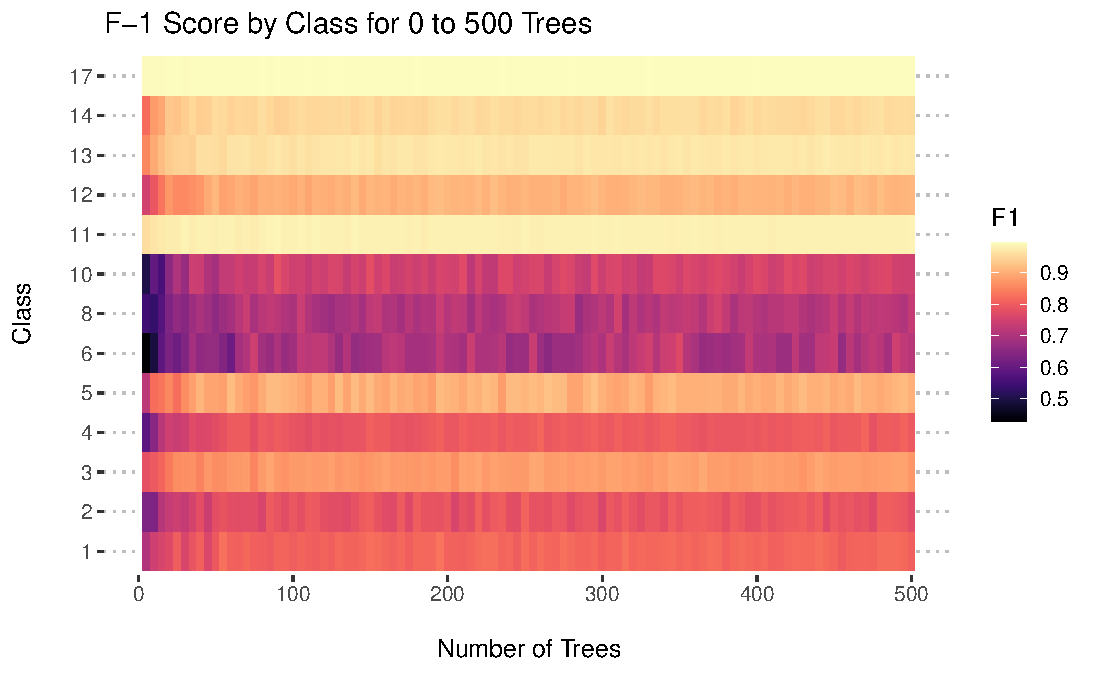
\includegraphics[width=0.75\linewidth]{../results/plots/ntree_5_to_500_heatmap} 

}

\caption{The variation between LCZ classes in F-1 score can be seen. As the number of trees in the random forest increases, F-1 score also increases, until around 100 trees. Note three approximate groupings of 1-5, 6-10, and 11-17. These metrics were calculated based on the out-of-bag dataset.}\label{fig:image-ref-for-in-text2}
\end{figure}

Almost all of the classes' F-1 scores appear to respond to increased
numbers of trees, to an extent. This response seems to stop entirely
once the number of trees reaches 100, but to explore it more thoroughly
I ran another simulation varying the number of trees between 25 and 2500
at intervals of 25. Increasing the number of trees has little to no
effect on the F-1 score by class (Figure 4).

\begin{figure}[H]

{\centering 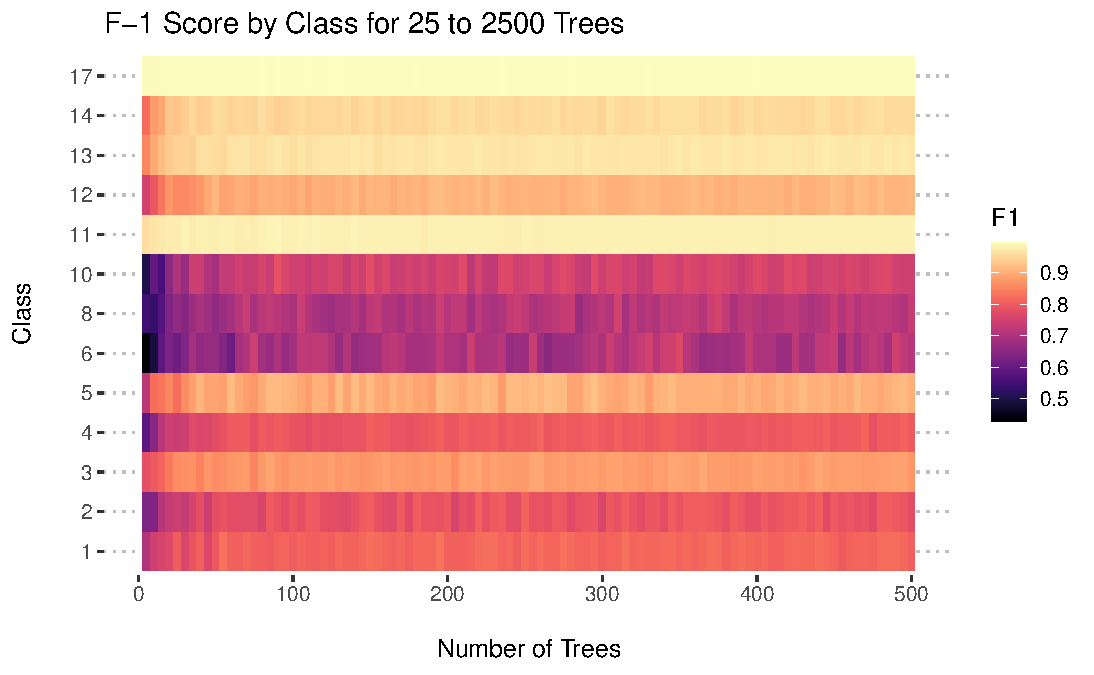
\includegraphics[width=0.75\linewidth]{../results/plots/ntree_25_to_2500_heatmap} 

}

\caption{The number of trees in the random forest does not seem to have a strong effect on the F-1 scores by class. This is based on the out-of-bag dataset and the number of trees was adjusted from 25 to 2500 in intervals of 25}\label{fig:image-ref-for-in-text3}
\end{figure}

\hypertarget{predicting-on-the-test-dataset}{%
\subsection{Predicting on the Test
Dataset}\label{predicting-on-the-test-dataset}}

\hypertarget{accuracy}{%
\subsubsection{Accuracy}\label{accuracy}}

Accuracy metrics dropped dramatically upon applying the random forest to
the test data (Figure 4). The F-1 Score for class 17, Water, remained
high, but since water has a very characteristic signature this is not
surprising. Classification for classes 2 (compact midrise), 5 (open
midrise), 8 (large low-rise), and 14 (low plants) performed especially
poorly.

\begin{figure}[H]

{\centering 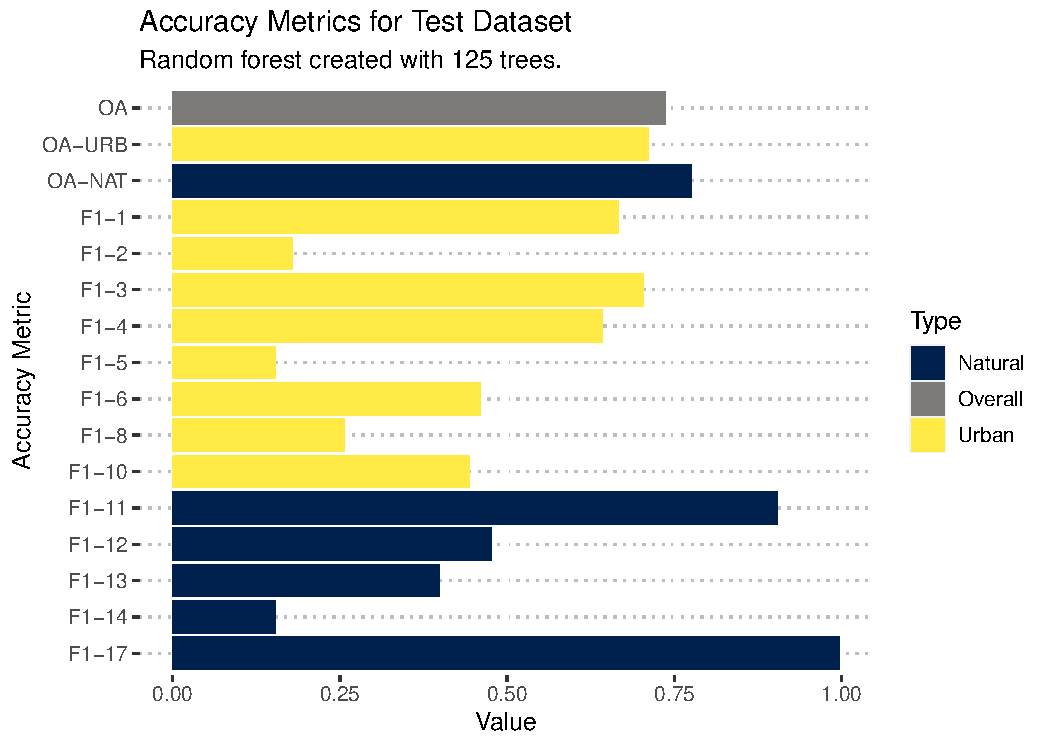
\includegraphics[width=0.75\linewidth]{../results/plots/test_set_accuracy_metrics_barplot} 

}

\caption{Accuracy among random forest predictions for the test dataset varied widely, but was overall lower than expected. Classes 2, 5, 8, and 14 have particularly low F-1 Scores}\label{fig:image-ref-for-in-text4}
\end{figure}

\hypertarget{importance-measures}{%
\subsubsection{Importance Measures}\label{importance-measures}}

In general there is not a clear pattern in which bands or scenes proved
to be the best predictors based on mean decrease in Gini Impurity
(Figure 5). However, bands 7, 10, and 11 in Scene 4 were particularly
useful. Scene 4 overall seems to contribute the most effectively to the
model, surpassing the other scenes in each of the bads except for 4,5,
and 6.

\begin{figure}[H]

{\centering 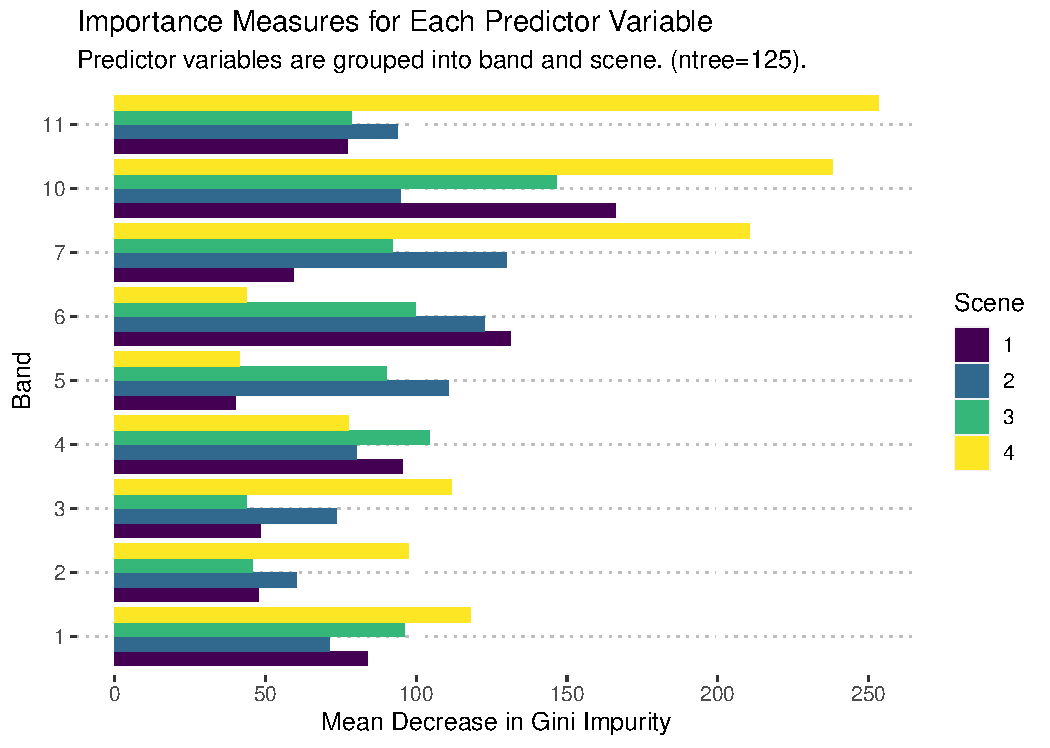
\includegraphics[width=0.75\linewidth]{../results/plots/importance_barplot_ntree125} 

}

\caption{There is not a clear pattern in Mean Decrease for Gini Impurity between the different bands and scenes, though there is some indication that bands in scene 4 were particularly effective as predictors.}\label{fig:image-ref-for-in-text5}
\end{figure}

\hypertarget{a-full-prediction}{%
\subsection{A Full Prediction}\label{a-full-prediction}}

Despite the decreased overall accuracy for the random forest based on
the test data, it is the best fitting model based on the training data,
and therefore the one I used for the full prediction of LCZ classes
throughout the Hong Kong area of interest (Figure 6).

\begin{figure}[H]

{\centering 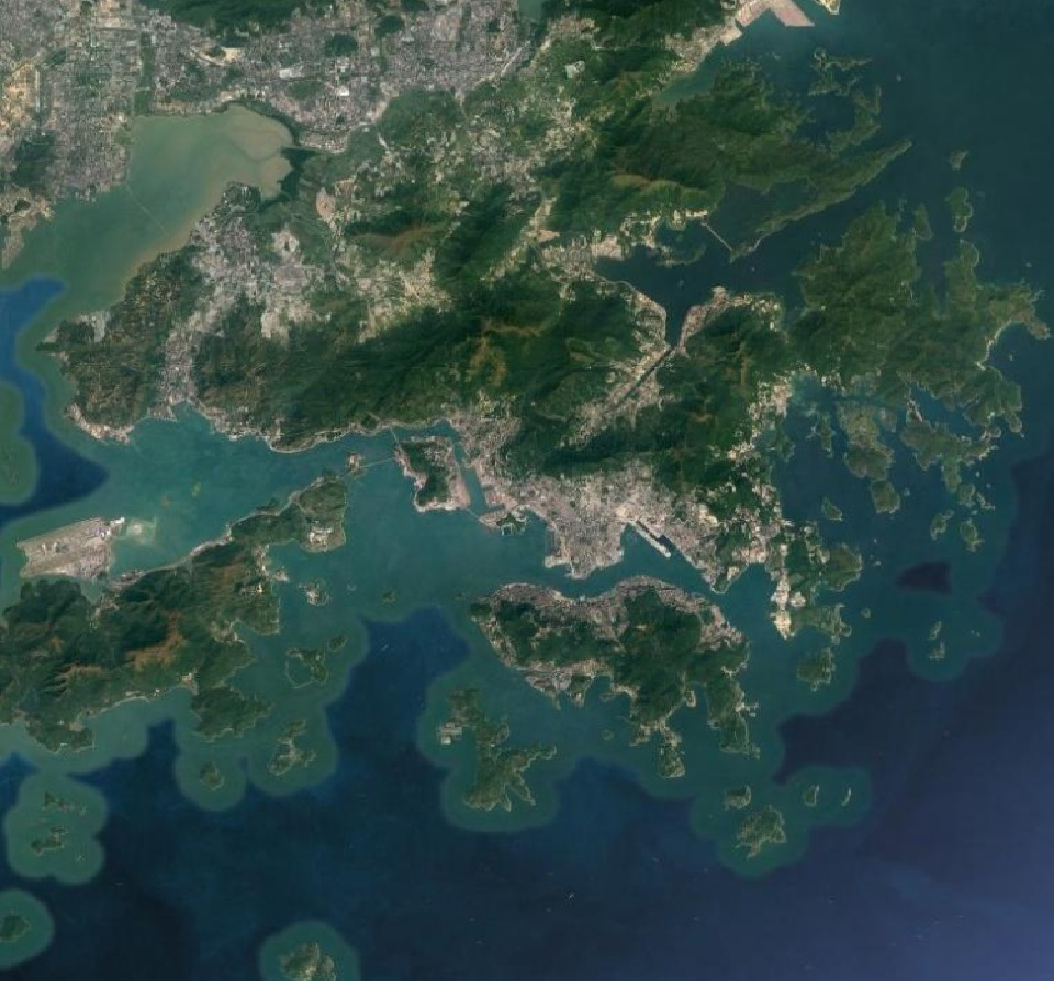
\includegraphics[width=0.45\linewidth]{../results/map_images/google_satellite} 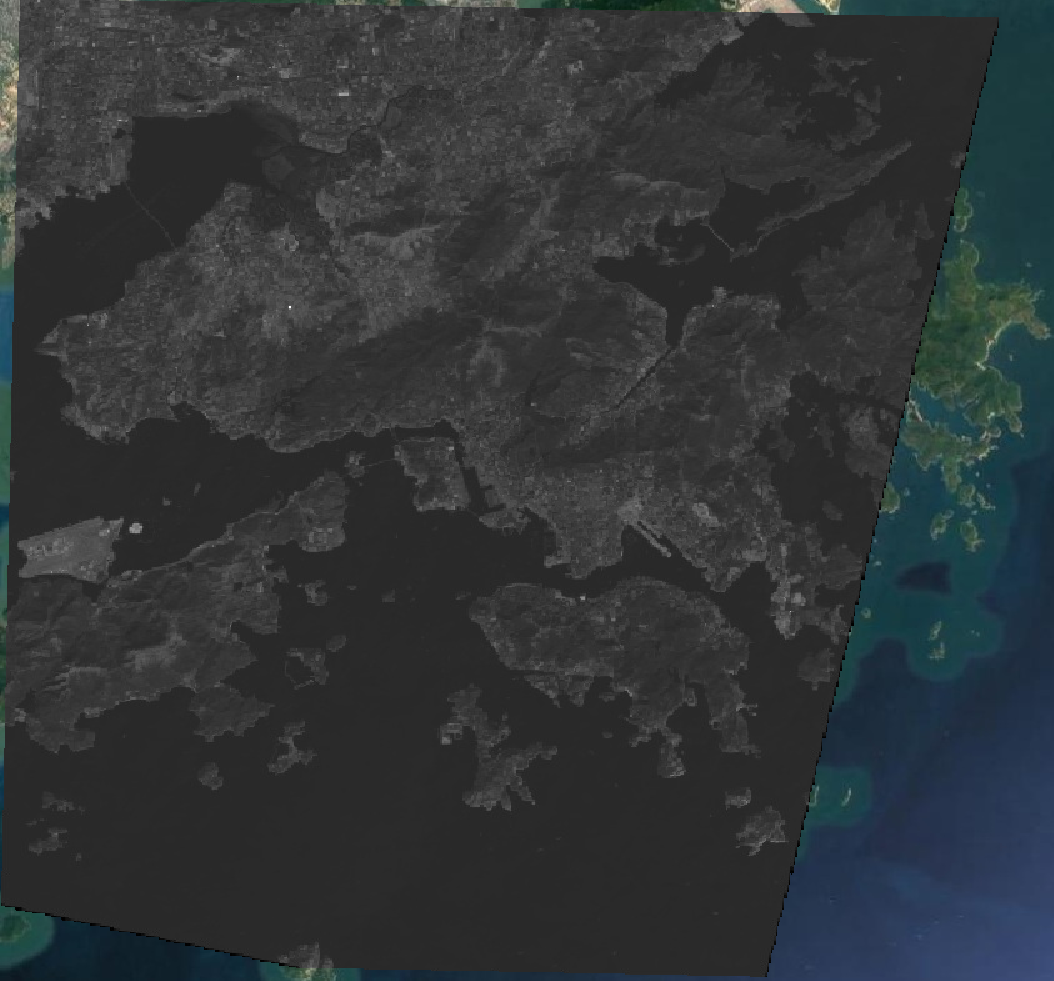
\includegraphics[width=0.45\linewidth]{../results/map_images/one_landsat_scene} 

}

\caption{landsat}\label{fig:maps1}
\end{figure}

\begin{figure}[H]

{\centering 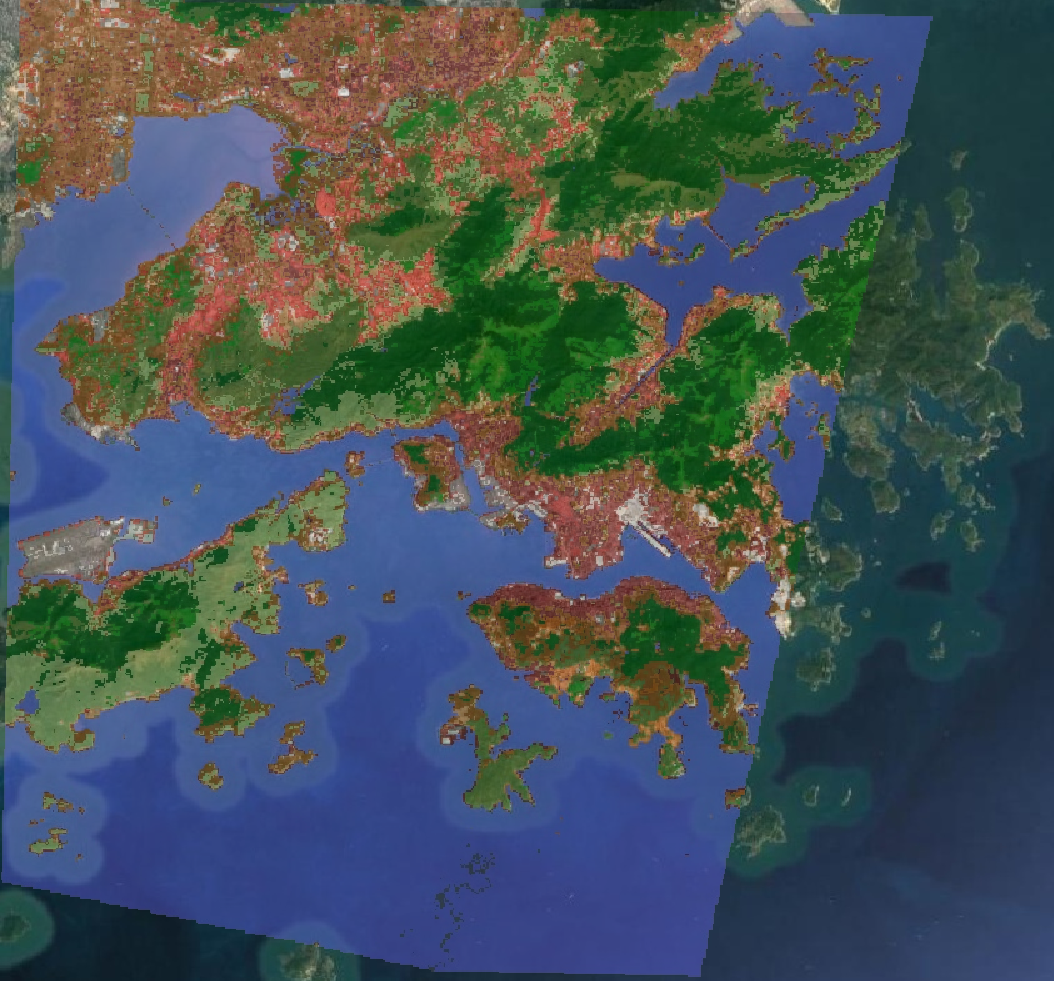
\includegraphics[width=0.5\linewidth]{../results/map_images/lcz_prediction} 

}

\caption{prediction}\label{fig:maps2}
\end{figure}

\hypertarget{discussion}{%
\section{Discussion}\label{discussion}}

The results of this analysis point to an issue in the current method for
using random forests to classify LCZ classes: Overall Accuracy can mask
very low F-1 scores in specific LCZ class categories. For example, water
has an accuracy of almost 100\% by every metric tested. It also takes up
a large proportion of the training and test data, as well as the overall
area of interest. As has been mentioned, the signature for water is
quite distinctive (CITE). Therefore it is reasonable to suggest that the
high rate of correct predictions is not due to the suitability of random
forest classification for LCZ classes, but rather it may be due to the
general ease of classifying water with Landsat 8 imagery, despite method
used.

That being said, there are a number of other reasons this discrepancy in
accuracy between classes could be occurring. The uneven distribution of
polygons in different classes in the training dataset is likely an
important contributor. The small proportion of training and test pixels
relative to the entire are of interest also may be cause for concern.
However, the latter is not actually tested for our accuracy methods due
to lack of a fully classified ground truth layer. Without this layer it
is not possible to test the transferability of these models to other
urban areas, but based on the classification success within Hong Kong,
it is likely that transferability is poor.

In terms of my results varying the parameters of the random forest,
there is an upper limit to how accurate the model can be. That upper
limit may be in part due to the appropriateness of the method, but I
postulate that the quality and amount of data is the true culprit. I
suggest this as an area for future study, as it would be valuable to
understand what level of initial classification commitment is necessary
for a robust LCZ analysis.

\newpage

\hypertarget{references}{%
\section{References}\label{references}}

\begin{itemize}
\tightlist
\item
  Bechtel, B., Alexander, P., Böhner, J., Ching, J., Conrad, O.,
  Feddema, J., Mills, G., See, L., \& Stewart, I. (2015). Mapping Local
  Climate Zones for a Worldwide Database of the Form and Function of
  Cities. ISPRS International Journal of Geo-Information, 4(1),
  199--219. \url{https://doi.org/10.3390/ijgi4010199}
\item
  Danylo, O., See, L., Bechtel, B., Schepaschenko, D., \& Fritz, S.
  (2016). Contributing to WUDAPT: A Local Climate Zone Classification of
  Two Cities in Ukraine. IEEE Journal of Selected Topics in Applied
  Earth Observations and Remote Sensing, 9(5), 1841--1853.
  \url{https://doi.org/10.1109/JSTARS.2016.2539977}
\item
  Demuzere, Matthias; Hankey, Steve; Mills, Gerald; Zhang, Wenwen; Lu,
  Tianjun; Bechtel, Benjamin (2020): CONUS-wide LCZ map and Training
  Areas. figshare. Dataset.
  \url{https://doi.org/10.6084/m9.figshare.11416950.v1}
\item
  Hibbard, K. A., Hoffman, F. M., Huntzinger, D., West, T. O., Wuebbles,
  D. J., Fahey, D. W., Hibbard, K. A., Dokken, D. J., Stewart, B. C., \&
  Maycock, T. K. (2017). Ch. 10: Changes in Land Cover and Terrestrial
  Biogeochemistry. Climate Science Special Report: Fourth National
  Climate Assessment, Volume I. U.S. Global Change Research Program.
  \url{https://doi.org/10.7930/J0416V6X}
\item
  Lempert, R. J., Arnold, J. R., Pulwarty, R. S., Gordon, K., Greig, K.,
  Hawkins-Hoffman, C., Sands, D., \& Werrell, C. (2018). Chapter 28:
  Adaptation Response. Impacts, Risks, and Adaptation in the United
  States: The Fourth National Climate Assessment, Volume II. U.S. Global
  Change Research Program. \url{https://doi.org/10.7930/NCA4.2018.CH28}
\item
  Santamouris, M. (2020). Recent progress on urban overheating and heat
  island research. Integrated assessment of the energy, environmental,
  vulnerability and health impact. Synergies with the global climate
  change. Energy and Buildings, 207, 109482.
  \url{https://doi.org/10.1016/j.enbuild.2019.109482}
\item
  Stewart, I. D., \& Oke, T. R. (2012). Local Climate Zones for Urban
  Temperature Studies. Bulletin of the American Meteorological Society,
  93(12), 1879--1900. \url{https://doi.org/10.1175/BAMS-D-11-00019.1}
\item
  Tuia, D., Moser, G., Le Saux, B., Bechtel, B., \& See, L. (2017). 2017
  IEEE GRSS Data Fusion Contest: Open Data for Global Multimodal Land
  Use Classification {[}Technical Committees{]}. IEEE Geoscience and
  Remote Sensing Magazine, 5(1), 70--73.
  \url{https://doi.org/10.1109/MGRS.2016.2645380}
\item
  United Nations, Department of Economic and Social Affairs, \&
  Population Division. (2019). World urbanization prospects: The 2018
  revision.
\item
  US EPA, O. (2014, June 17). Heat Island Impacts {[}Overviews and
  Factsheets{]}. US EPA.
  \url{https://www.epa.gov/heatislands/heat-island-impacts}
\item
  Verdonck, M.-L., Okujeni, A., van der Linden, S., Demuzere, M., De
  Wulf, R., \& Van Coillie, F. (2017). Influence of neighbourhood
  information on `Local Climate Zone' mapping in heterogeneous cities.
  International Journal of Applied Earth Observation and Geoinformation,
  62, 102--113. \url{https://doi.org/10.1016/j.jag.2017.05.017}
\item
  Yokoya, N., Ghamisi, P., Xia, J., Sukhanov, S., Heremans, R.,
  Tankoyeu, I., Bechtel, B., Saux, B. L., \& Moser, G. (2018). Open Data
  for Global Multimodal Land Use Classification: Outcome of the 2017
  IEEE GRSS Data Fusion Contest. IEEE Journal of Selected Topics in
  Applied Earth Observations and Remote Sensing, 11(5), 15.
\item
  Yoo, C., Han, D., Im, J., \& Bechtel, B. (2019). Comparison between
  convolutional neural networks and random forest for local climate zone
  classification in mega urban areas using Landsat images. ISPRS Journal
  of Photogrammetry and Remote Sensing, 157, 155--170.
  \url{https://doi.org/10.1016/j.isprsjprs.2019.09.009}
\item
  Zhen, Z., Quackenbush, L. J., Stehman, S. V., \& Zhang, L. (2013).
  Impact of training and validation sample selection on classification
  accuracy and accuracy assessment when using reference polygons in
  object-based classification. International Journal of Remote Sensing,
  34(19), 6914--6930. \url{https://doi.org/10.1080/01431161.2013.810822}
\end{itemize}

\end{document}
